\documentclass{article}
\usepackage[T1]{fontenc}
\usepackage{lmodern}
\usepackage{graphicx}
\usepackage{amsmath,amssymb}
\usepackage[a4paper,margin=2cm]{geometry}
\usepackage[absolute,overlay]{textpos}
\setlength{\TPHorizModule}{1mm}
\setlength{\TPVertModule}{1mm}
\usepackage[indonesian]{babel}
\usepackage{hyperref}
\setlength{\emergencystretch}{2em}
% unit: Halaman 48

\begin{document}

% === Halaman 48 (llm) ===

\vspace{92.07mm}

\section*{Operasi RC4 secara keseluruhan:}

\vspace{130.68mm}

% deskripsi: Diagram proses inisialisasi state dan kunci RC4, mencakup tahap 'State and key initialization' dan 'Initial state permutation'.
% bbox normalisasi: [0.2100, 0.1700, 0.6600, 0.4800]
\begin{textblock*}{94.50mm}(44.10mm,50.49mm)
\noindent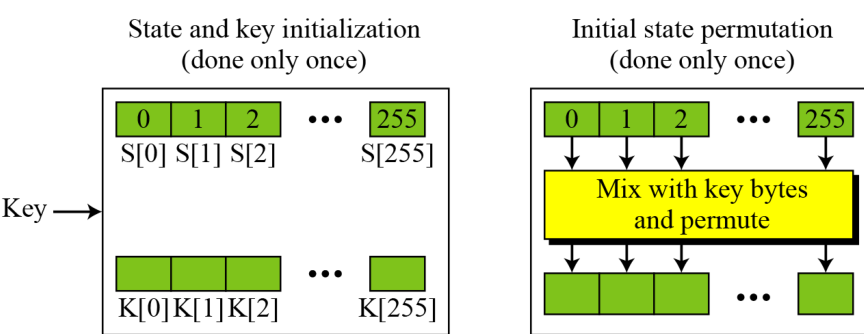
\includegraphics[width=94.50mm,height=92.07mm]{../../images/llm/page_048_img_01.png}%
\end{textblock*}

% deskripsi: Diagram proses pembuatan key stream RC4 melalui 'State permutation for key stream generation' dan operasi enkripsi XOR antara plaintext (P) dan key stream (k) untuk menghasilkan ciphertext (C).
% bbox normalisasi: [0.1100, 0.5400, 0.7300, 0.9800]
\begin{textblock*}{130.20mm}(23.10mm,160.38mm)
\noindent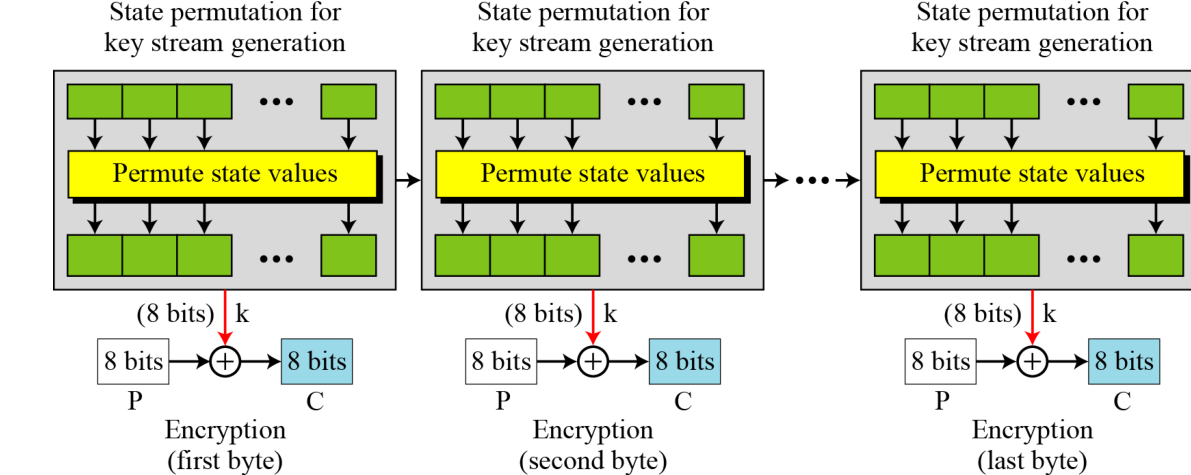
\includegraphics[width=130.20mm,height=130.68mm]{../../images/llm/page_048_img_02.png}%
\end{textblock*}

\end{document}
